204. \begin{figure}[ht!]
\center{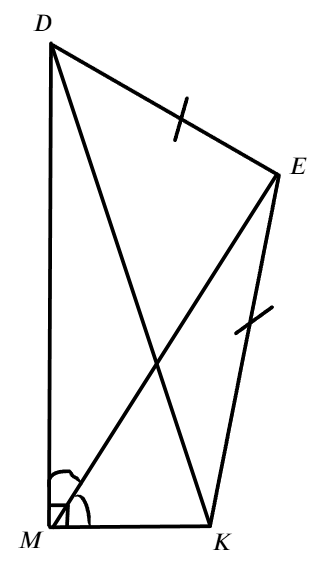
\includegraphics[scale=0.35]{g9-202.png}}
\end{figure}\\
Так как $ME$ является биссектрисой, $\angle DME=\angle KME=90^\circ:2=45^\circ.$ Пусть $MK=x,$ тогда $MD=7x$ и по теореме косинусов для треугольника $DME$ имеет место соотношение $DE^2=49x^2+16-56x\cdot \cfrac{\sqrt{2}}{2},\ DE^2=16+49x^2-28\sqrt{2}x.$ По теореме косинусов для треугольника $EMK$ имеет место равенство $EK^2=x^2+16-8x\cdot \cfrac{\sqrt{2}}{2},\ EK^2=16+x^2-4\sqrt{2}x.$ Так как $DE=EK,$ получим равенство $16+49x^2-28\sqrt{2}x=16+x^2-4\sqrt{2}x,\ 48x^2=24\sqrt{2}x,\ 2x=\sqrt{2},\ x=\cfrac{\sqrt{2}}{2}.$ Тогда $DK=\sqrt{x^2+49x^2}=\sqrt{50x^2}=\sqrt{25}=5.$\\
